\chapter{Architecture}
% OR: \chapter{Model}
\label{cha:architecture}

\begin{comment}
Here you will present the architecture or model that you have chosen and which is (or will be) implemented in your work.
Note that putting algorithms in your report is not always desirable, so in certain cases those might be placed in the appendix.
Code is normally to be avoided in the report itself, but may be included in an appendix or submitted as additional documents.
(The actual code must also be submitted together with the final Master's thesis, but as a zip-file.)

Any off-the-shelf tools and methods that you use in your architecture should have been introduced earlier,
tentatively in the Background chapter (or in the Related Work chapter),
so that they can be referenced here by giving backward pointers to the previous text.

Here, or in a separate chapter (or possibly in the Background chapter or in the Experimental Setup),
you should also discuss the data that you use in your experiments (see Chapter~\ref{cha:data}).

\textit{Nunc in tristique risus, ut malesuada tortor. Integer ullamcorper nunc a felis vehicula condimentum. Aliquam eget turpis purus. Nam nec ipsum sed ligula vulputate tempor ac non arcu. Aenean hendrerit pretium ante et suscipit. Proin vitae venenatis ex, at pellentesque erat. Nulla facilisi. Sed quis eros lorem. Praesent id pharetra risus. Nunc a lacinia est. Nunc in urna at purus ullamcorper blandit eget sit amet est. Cras sagittis et ante ut lobortis. Proin quis arcu eros. Aliquam tempor neque vehicula lacus placerat, ac ultricies massa ultricies. Aliquam et nulla eget felis accumsan rutrum quis sed ligula.}

\textit{Vivamus bibendum tempus tincidunt. Integer imperdiet lectus pellentesque, rhoncus quam at, tempor ex. Phasellus semper tempor sapien at consequat. Proin ut dolor interdum, ullamcorper leo ac, convallis metus. Nullam tincidunt, metus ullamcorper sodales placerat, ipsum ipsum porttitor est, id volutpat orci orci sit amet quam. Vestibulum sagittis urna sit amet nulla vulputate, nec pellentesque enim hendrerit. Suspendisse at laoreet ipsum. Phasellus arcu nisi, laoreet sed tellus sit amet, imperdiet fringilla ante. Quisque rhoncus accumsan magna vel posuere. Fusce facilisis est eros, ac viverra diam maximus ut. Nullam ut lectus nunc. Fusce vestibulum sem at ex euismod tempus. Lorem ipsum dolor sit amet, consectetur adipiscing.}

\textit{Phasellus sed ipsum nunc. Nam iaculis felis mauris, sit amet condimentum ex malesuada at. Morbi lacinia odio mi, sit amet pellentesque ante facilisis sit amet. In lobortis elit ut dictum mollis. Aliquam erat volutpat. Morbi sit amet metus nisi. Nulla auctor varius metus at rhoncus. Pellentesque porta mollis leo, eu ultricies nulla mollis ac. Vivamus interdum ac odio vitae sodales. Aenean finibus eros rhoncus molestie elementum. Integer maximus erat vitae purus lobortis iaculis. Etiam blandit varius nulla, sed euismod felis.}

Clearly, a figure showing the architecture is a must, such as Figure~\ref{fig:Architecture}.
Describe all parts of such a figure in reasonable detail in the text, possibly with forward pointers to sections where they will be elaborated on (or backward pointers to sections where tools and methods already have been introduced).
Mention work that motivated your architectural choices, parameter settings, etc.
Those choices should then also be discussed and elaborated on in the Discussion chapter.

\begin{figure}[t!]
    \centering
    \missingfigure{Architecture figure to be added}
    \caption{The missing architecture}
    \label{fig:Architecture}
\end{figure}
\end{comment}

\section{High-Level Application Architecture}

A microservice architecture was employed in order to simplify development and separate concerns between the different microservices. The services are deployed as Docker Containers, and they are orchestrated using Docker Compose. \autoref{fig:architecture-overview} shows how the application is divided into five distinct services.

\begin{figure}[h]
    \centering
    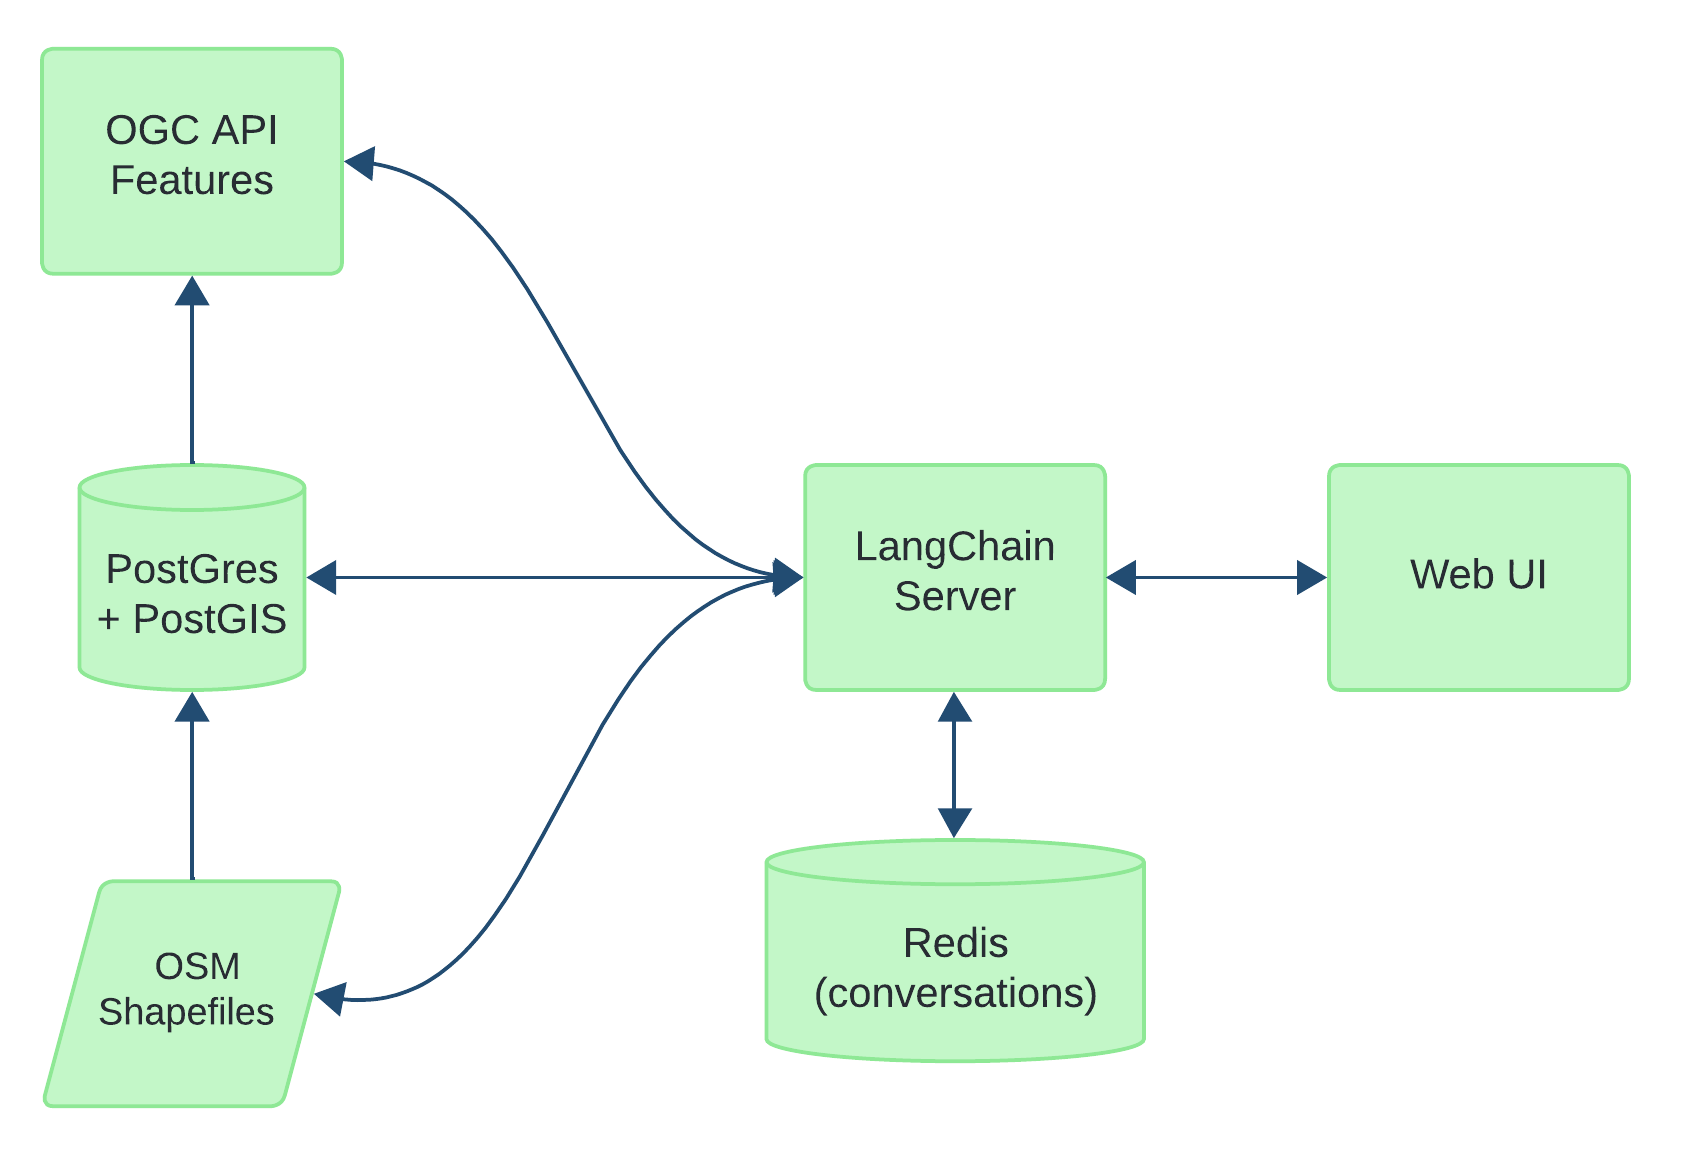
\includegraphics[width=\textwidth]{microservices.png}
    \caption{Architecture overview}
    \label{fig:architecture-overview}
\end{figure}

The \textit{LangChain server} is the heart of the application, and is where the \gls{acr:llm}-related logic is situated.

\section{LangChain Server}\label{sec:langchain}

LangChain \citep{chaseLangChain2022} is an open-source project that provides tooling that can be used to create autonomous \acrshort{acr:ai} agents. It is designed to help with prompt management and optimization, creating chains of calls to \acrshortpl{acr:llm}, data-augmented generation, autonomous agent creation, and memory-related tasks.

LangGraph is nice.

\section{Redis for Conversations}
\section{PostGres + PostGIS}
\section[OGC API Features]{\acrshort{acr:ogc} \acrshort{acr:api} Features}
\section[Web UI]{Web \acrshort{acr:ui}}


\glsresetall

